\chapter{Implementaci\'on}
\label{cap:implementacion}

\section{Desarrollo de la aplicación}
Dentro del campo de procesamiento de textos, el análisis de letras de canciones no es el más popular, sin embargo existen algunos trabajos que nos han servido de guía para establecer los límites y punto de comienzo de nuestro proyecto. Sin duda el proyecto existente que más se ajusta a nuestra primera idea es \href{https://medium.com/@alexing/data-data-b82201ec1cf4}{\textit{Data, data}}, que hace un estudio exahustivo de las canciones del cantante Uruguayo Jorge Drexler, tanto de la letra como de la música.

Como hemos comentado en el Capítulo 2, nuestros objetivos son obtener los sentimientos que predominan en diferentes países, y comprobar si la hipótesis que hemos establecido indicando que el tema dominante en España es el amor.

\section{Creación del conjunto de datos}
Nuestro punto de partida son los datos que encontramos en varios datasets de Kaggle \footnote{\url{https://www.kaggle.com/mousehead/songlyrics }} \footnote{\url{https://www.kaggle.com/gyani95/380000-lyrics-from-metrolyrics}}. Cuyo formato, en el primer caso, es el que se aprecia en la Figura \ref{fig:dataset1}. Se componede 4 columnas, la primera contiene el nombre del grupo, la segunda el título de la canción, seguida en la siguiente columna de un link que unido a http://www.lyricsfreak.com/ nos redirige a una página donde encontramos más información de la canción, como el año de publicación entre otros, y por último la letra.
\begin{figure}
	\centering
	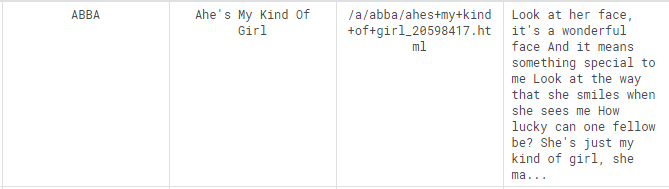
\includegraphics[width=0.7\linewidth]{Imagenes/dataset1}
	\caption{}
	\label{fig:dataset1}
\end{figure}
En el caso del segundo dataset, el formato es el que se aprecia en la Figura \ref{fig:dataset2}. En él encontramos el nombre del grupo, seguido del año de publicación de la canción, cuyo nombre aparece en la tercera columna, y finalmente la letra.
\begin{figure}
	\centering
	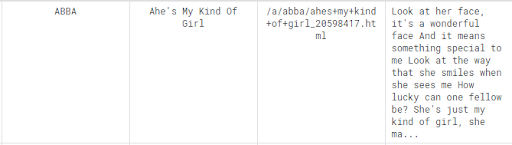
\includegraphics[width=0.7\linewidth]{Imagenes/dataset2}
	\caption{}
	\label{fig:dataset2}
\end{figure}

Un dato relevante en el desarrollo de ésta práctica del cual no disponemos a través de Kaggle es el país de procedencia de cada autor(a). Para obtenerlo utilizaremos técnicas de minería web para extraer dicha información a través de Wikipedia u otras fuentes. Una vez obtenida la información (país, autor, letras de sus canciones), limpiaremos los datos escogiendo sólo las palabras más relevantes, siendo éstas los verbos, sustantivos y adjetivos, eliminando artículos, conjunciones.

\section{Limpieza y preprocesamiento de los datos}
La limpiza de las letras es un paso crucial en el desarrollo de éste proyecto, puesto que muchas letras están compuestas de palabras que no aportan información relevante a la hora de realizar el análisis, como son los artículos, conjunciones, etc. Por ello, una vez obtenidos todos los datos, el paso siguiente será eliminar las llamadas \textit{stopwords}, tanto del inglés como del castellano. Éste conjunto de palabras está compuesto por los tipos comentados anteriormente, es decir, palabras que no aportan información al análisis. Para ello, hemos desarrollado una función en R que, dado un texto, extrae únicamente las palabras que se encuentran en el diccionario, tanto en el de inglés como en el de castellano.

Como parte del preprocesamiento de los datos y con el fin de obtener una descripción más visual del set de datos obtenido, hemos realizado algunas pruebas. En primer lugar, hemos obtenido las palabras que aparecen en las canciones más conocidas del grupo Queen.
\begin{figure}[h]
	\centering
	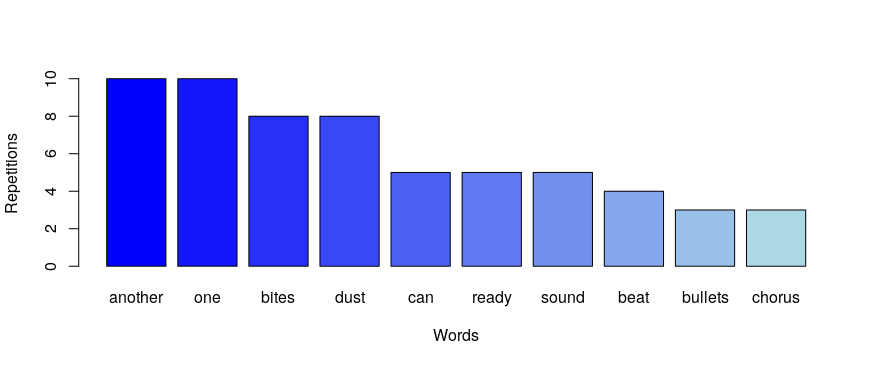
\includegraphics[width=0.7\linewidth]{Imagenes/AnotherOneBitesTheDust}
	\caption{\textit{Another One Bites the Dust} - Queen}
	\label{fig:AnotherOneBitesTheDust}
\end{figure}
\begin{figure}[h]
	\centering
	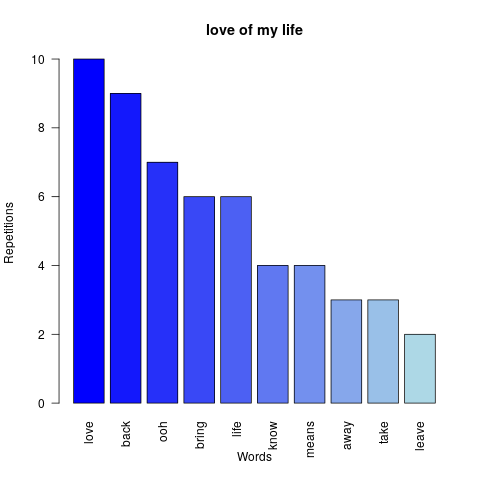
\includegraphics[width=0.7\linewidth]{Imagenes/loveofmylife}
	\caption{\textit{Love Of My life} - Queen}
	\label{fig:loveofmylife}
\end{figure}
\begin{figure}[h]
	\centering
	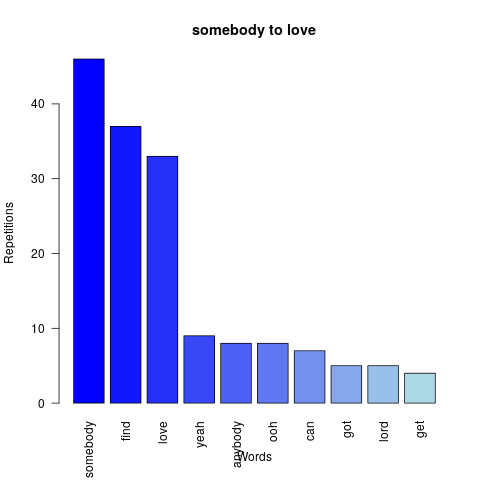
\includegraphics[width=0.7\linewidth]{Imagenes/somebodytolove}
	\caption{\textit{Somebody To Love} - Queen}
	\label{fig:sbtl}	
\end{figure}
\begin{figure}[h]
	\centering
	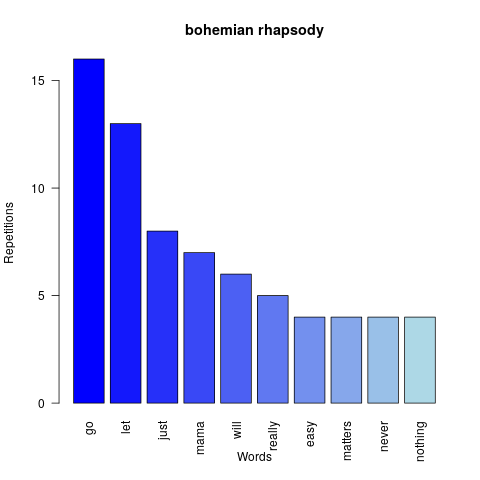
\includegraphics[width=0.7\linewidth]{Imagenes/bohemianrhapsody}
	\caption{\textit{Bohemian Rhapsody} - Queen}
	\label{fig:bohemianrhapsody}
\end{figure}
\begin{figure}[h]
	\centering
	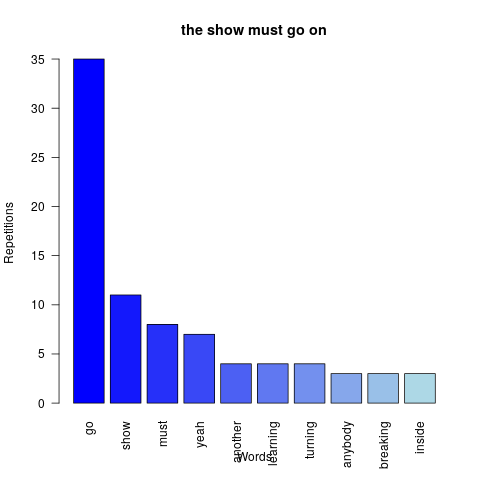
\includegraphics[width=0.7\linewidth]{Imagenes/theshowmustgoon}
	\caption{\textit{The Show must go on} - Queen}
	\label{fig:tsmgo}
\end{figure}

Finalmente, tras estudiar los gráficos obtenidos y ver que tiene sentido que las palabras más utilizadas en dichas canciones son las que se muestran, procedemos a generalizar un poco más nuestra exploración, para ver cuales son las palabras más utilizadas por el grupo británico. Como se muestra en la figura \ref{fig:queen_songs}, la palabra \textit{amor} aparece más de 400 veces en las canciones de las que disponemos de dicha banda.
\begin{figure}[h]
	\centering
	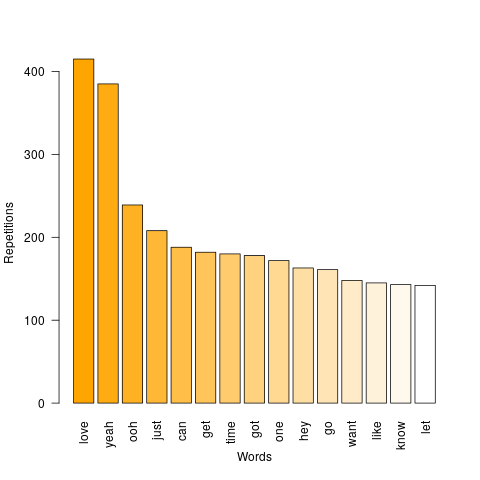
\includegraphics[width=0.7\linewidth]{Imagenes/queen_most_used_words}
	\caption{Most used words by Queen}
	\label{fig:queen_songs}
\end{figure}

\section{Transformación de los datos}
\section{Elección de la tarea de minado adecuada}
\section{Eleección del algoritmo de minería de datos}
\section{Aplicación del algoritmo elegido}
\section{Interpretación de los resultados}
\section{Aplicación de los resultados obtenidos}